\section{Nano-Scale Flow}
\label{sec:nano}

\begin{frame}
    \frametitle{Nano-Scale flow}
    
    \begin{columns}
        \begin{column}{0.3\textwidth}
            \begin{itemize}
                \item We ran 5 simulations
                \item Base simulation did not generate directed flow
                \item After setting $\sigma = 0.8$, $\epsilon = 5.0$, and $g_{grav}=-9.81$, we obtained a nice result
            \end{itemize}

            \vspace{7pt}
            \hrule
            \vspace{7pt}

            \begin{itemize}
                \item Particles are immobilized by type
                \item Analytics are measured in multiple dimensions
                \item Python script can generate profile from vtk
            \end{itemize}
        \end{column}
        \begin{column}{.7\textwidth}
            \begin{figure}
                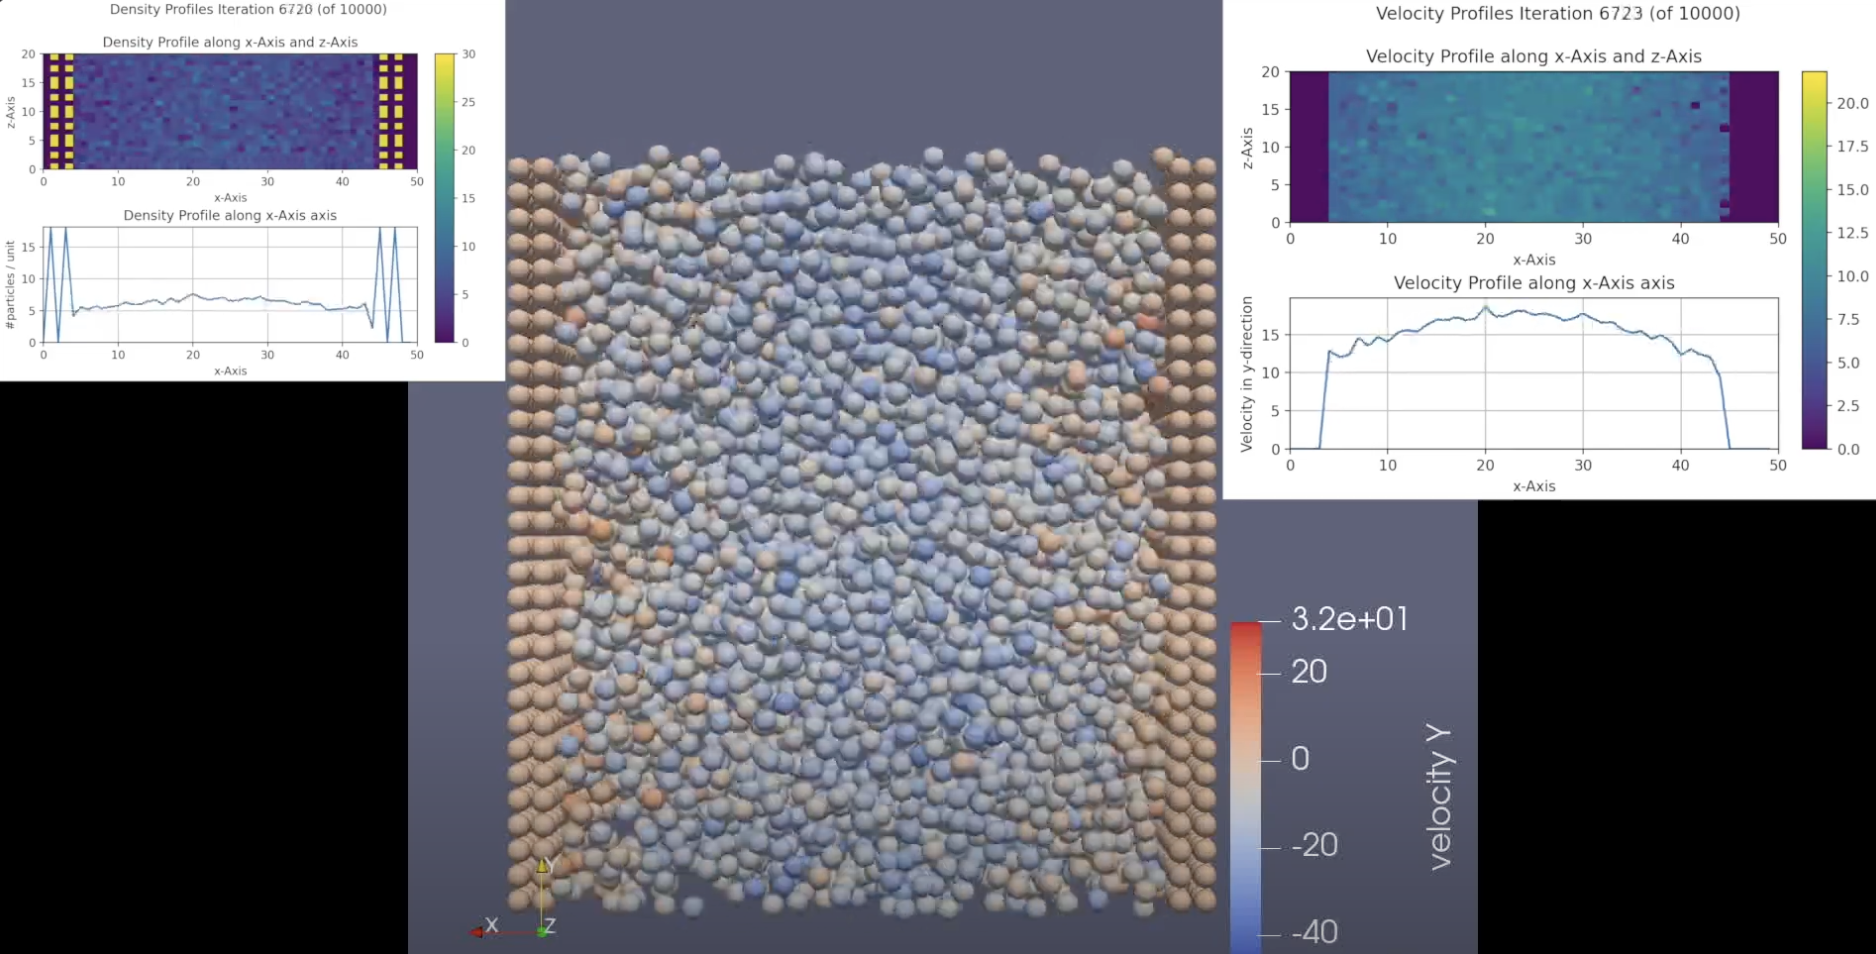
\includegraphics[width=\columnwidth]{../../res/Stronger_walls_nano_flow.png}
                \caption{Stronger wall slows particles on the borders while gravity accelerates the center. Thermostat will ignore mean velocity. }
                \label{fig:strong-walls}
            \end{figure}
        \end{column}
    \end{columns}
    
    
\end{frame}